% Options for packages loaded elsewhere
\PassOptionsToPackage{unicode}{hyperref}
\PassOptionsToPackage{hyphens}{url}
\PassOptionsToPackage{dvipsnames,svgnames,x11names}{xcolor}
%
\documentclass[
]{article}
\usepackage{amsmath,amssymb}
\usepackage{iftex}
\ifPDFTeX
  \usepackage[T1]{fontenc}
  \usepackage[utf8]{inputenc}
  \usepackage{textcomp} % provide euro and other symbols
\else % if luatex or xetex
  \usepackage{unicode-math} % this also loads fontspec
  \defaultfontfeatures{Scale=MatchLowercase}
  \defaultfontfeatures[\rmfamily]{Ligatures=TeX,Scale=1}
\fi
\usepackage{lmodern}
\ifPDFTeX\else
  % xetex/luatex font selection
\fi
% Use upquote if available, for straight quotes in verbatim environments
\IfFileExists{upquote.sty}{\usepackage{upquote}}{}
\IfFileExists{microtype.sty}{% use microtype if available
  \usepackage[]{microtype}
  \UseMicrotypeSet[protrusion]{basicmath} % disable protrusion for tt fonts
}{}
\makeatletter
\@ifundefined{KOMAClassName}{% if non-KOMA class
  \IfFileExists{parskip.sty}{%
    \usepackage{parskip}
  }{% else
    \setlength{\parindent}{0pt}
    \setlength{\parskip}{6pt plus 2pt minus 1pt}}
}{% if KOMA class
  \KOMAoptions{parskip=half}}
\makeatother
\usepackage{xcolor}
\usepackage[margin=1in]{geometry}
\usepackage{color}
\usepackage{fancyvrb}
\newcommand{\VerbBar}{|}
\newcommand{\VERB}{\Verb[commandchars=\\\{\}]}
\DefineVerbatimEnvironment{Highlighting}{Verbatim}{commandchars=\\\{\}}
% Add ',fontsize=\small' for more characters per line
\usepackage{framed}
\definecolor{shadecolor}{RGB}{248,248,248}
\newenvironment{Shaded}{\begin{snugshade}}{\end{snugshade}}
\newcommand{\AlertTok}[1]{\textcolor[rgb]{0.94,0.16,0.16}{#1}}
\newcommand{\AnnotationTok}[1]{\textcolor[rgb]{0.56,0.35,0.01}{\textbf{\textit{#1}}}}
\newcommand{\AttributeTok}[1]{\textcolor[rgb]{0.13,0.29,0.53}{#1}}
\newcommand{\BaseNTok}[1]{\textcolor[rgb]{0.00,0.00,0.81}{#1}}
\newcommand{\BuiltInTok}[1]{#1}
\newcommand{\CharTok}[1]{\textcolor[rgb]{0.31,0.60,0.02}{#1}}
\newcommand{\CommentTok}[1]{\textcolor[rgb]{0.56,0.35,0.01}{\textit{#1}}}
\newcommand{\CommentVarTok}[1]{\textcolor[rgb]{0.56,0.35,0.01}{\textbf{\textit{#1}}}}
\newcommand{\ConstantTok}[1]{\textcolor[rgb]{0.56,0.35,0.01}{#1}}
\newcommand{\ControlFlowTok}[1]{\textcolor[rgb]{0.13,0.29,0.53}{\textbf{#1}}}
\newcommand{\DataTypeTok}[1]{\textcolor[rgb]{0.13,0.29,0.53}{#1}}
\newcommand{\DecValTok}[1]{\textcolor[rgb]{0.00,0.00,0.81}{#1}}
\newcommand{\DocumentationTok}[1]{\textcolor[rgb]{0.56,0.35,0.01}{\textbf{\textit{#1}}}}
\newcommand{\ErrorTok}[1]{\textcolor[rgb]{0.64,0.00,0.00}{\textbf{#1}}}
\newcommand{\ExtensionTok}[1]{#1}
\newcommand{\FloatTok}[1]{\textcolor[rgb]{0.00,0.00,0.81}{#1}}
\newcommand{\FunctionTok}[1]{\textcolor[rgb]{0.13,0.29,0.53}{\textbf{#1}}}
\newcommand{\ImportTok}[1]{#1}
\newcommand{\InformationTok}[1]{\textcolor[rgb]{0.56,0.35,0.01}{\textbf{\textit{#1}}}}
\newcommand{\KeywordTok}[1]{\textcolor[rgb]{0.13,0.29,0.53}{\textbf{#1}}}
\newcommand{\NormalTok}[1]{#1}
\newcommand{\OperatorTok}[1]{\textcolor[rgb]{0.81,0.36,0.00}{\textbf{#1}}}
\newcommand{\OtherTok}[1]{\textcolor[rgb]{0.56,0.35,0.01}{#1}}
\newcommand{\PreprocessorTok}[1]{\textcolor[rgb]{0.56,0.35,0.01}{\textit{#1}}}
\newcommand{\RegionMarkerTok}[1]{#1}
\newcommand{\SpecialCharTok}[1]{\textcolor[rgb]{0.81,0.36,0.00}{\textbf{#1}}}
\newcommand{\SpecialStringTok}[1]{\textcolor[rgb]{0.31,0.60,0.02}{#1}}
\newcommand{\StringTok}[1]{\textcolor[rgb]{0.31,0.60,0.02}{#1}}
\newcommand{\VariableTok}[1]{\textcolor[rgb]{0.00,0.00,0.00}{#1}}
\newcommand{\VerbatimStringTok}[1]{\textcolor[rgb]{0.31,0.60,0.02}{#1}}
\newcommand{\WarningTok}[1]{\textcolor[rgb]{0.56,0.35,0.01}{\textbf{\textit{#1}}}}
\usepackage{longtable,booktabs,array}
\usepackage{calc} % for calculating minipage widths
% Correct order of tables after \paragraph or \subparagraph
\usepackage{etoolbox}
\makeatletter
\patchcmd\longtable{\par}{\if@noskipsec\mbox{}\fi\par}{}{}
\makeatother
% Allow footnotes in longtable head/foot
\IfFileExists{footnotehyper.sty}{\usepackage{footnotehyper}}{\usepackage{footnote}}
\makesavenoteenv{longtable}
\usepackage{graphicx}
\makeatletter
\newsavebox\pandoc@box
\newcommand*\pandocbounded[1]{% scales image to fit in text height/width
  \sbox\pandoc@box{#1}%
  \Gscale@div\@tempa{\textheight}{\dimexpr\ht\pandoc@box+\dp\pandoc@box\relax}%
  \Gscale@div\@tempb{\linewidth}{\wd\pandoc@box}%
  \ifdim\@tempb\p@<\@tempa\p@\let\@tempa\@tempb\fi% select the smaller of both
  \ifdim\@tempa\p@<\p@\scalebox{\@tempa}{\usebox\pandoc@box}%
  \else\usebox{\pandoc@box}%
  \fi%
}
% Set default figure placement to htbp
\def\fps@figure{htbp}
\makeatother
\setlength{\emergencystretch}{3em} % prevent overfull lines
\providecommand{\tightlist}{%
  \setlength{\itemsep}{0pt}\setlength{\parskip}{0pt}}
\setcounter{secnumdepth}{-\maxdimen} % remove section numbering
\usepackage{fancyhdr}
\pagestyle{fancy}
\fancyhf{}
\lfoot[\thepage]{}
\rfoot[]{\thepage}
\fontsize{12}{22}
\selectfont
\usepackage{bookmark}
\IfFileExists{xurl.sty}{\usepackage{xurl}}{} % add URL line breaks if available
\urlstyle{same}
\hypersetup{
  colorlinks=true,
  linkcolor={blue},
  filecolor={Maroon},
  citecolor={Blue},
  urlcolor={Blue},
  pdfcreator={LaTeX via pandoc}}

\title{\includegraphics[width=6cm,height=\textheight,keepaspectratio]{figures/IEO-logo.jpg}}
\author{}
\date{\vspace{-2.5em}}

\begin{document}
\maketitle


\pagenumbering{gobble}

%\begin{titlepage}
\begin{flushleft}
\Large{\textbf{Supplementary Material 1}}\\
\vspace*{2\baselineskip}
\LARGE{\textbf{Evaluating the effects of varying minimum legal sizes on population variables in the wedge clam \textit{Donax trunculus} fishery using an integrated model}}\\
\vspace*{5\baselineskip}
\Large{Project FEMP 04}\\
\vspace*{1\baselineskip}
\Large{Instituto Español de Oceanografía, Cádiz }\\
\vspace*{4\baselineskip}
\end{flushleft}
\begin{flushright}
\large{\textit{Mauricio Mardones}}\\
\large{\textit{Marina Delgado}}\\
\vspace*{1\baselineskip}
\normalsize{\textbf{Fecha}}\\
Abril, 2024
\end{flushright}

% \end{titlepage}


\hypersetup{linkcolor = black}
\newpage
\pagenumbering{roman}
%\tableofcontents
%\addcontentsline{toc}{section}{\contentsname}

\newpage



\pagenumbering{arabic}
\hypersetup{linkcolor = blue}

{
\hypersetup{linkcolor=}
\setcounter{tocdepth}{3}
\tableofcontents
}
\pagebreak

\section{Análisis de Vientos de Levante y Poniente}\label{anuxe1lisis-de-vientos-de-levante-y-poniente}

Este documento presenta un análisis comprensivo de los patrones de viento de Levante y Poniente basado en datos meteorológicos del período 2013-2025. El análisis incluye la caracterización temporal, intensidad y duración de estos eventos atmosféricos.

El objetivo de este trabajo es encontrar y cuantificar los patrones de viento y relacionarlos con variables poblacionales de Coquina \emph{Donax trunculus} provenientes del monitoreo poblacional y pesquero que lleva a cabo el IEO en el marco del proyecto FEMP 04.

\subsection{Carga de librerías y datos}\label{carga-de-libreruxedas-y-datos}

\begin{Shaded}
\begin{Highlighting}[]
\CommentTok{\# Vector con todos los paquetes que}
\CommentTok{\# necesitas}
\NormalTok{paquetes }\OtherTok{\textless{}{-}} \FunctionTok{c}\NormalTok{(}\StringTok{"readr"}\NormalTok{, }\StringTok{"dplyr"}\NormalTok{, }\StringTok{"lubridate"}\NormalTok{,}
    \StringTok{"stringr"}\NormalTok{, }\StringTok{"purrr"}\NormalTok{, }\StringTok{"ggplot2"}\NormalTok{, }\StringTok{"tidyr"}\NormalTok{,}
    \StringTok{"gridExtra"}\NormalTok{, }\StringTok{"viridis"}\NormalTok{, }\StringTok{"scales"}\NormalTok{, }\StringTok{"formatR"}\NormalTok{)}

\NormalTok{purrr}\SpecialCharTok{::}\FunctionTok{walk}\NormalTok{(paquetes, library, }\AttributeTok{character.only =} \ConstantTok{TRUE}\NormalTok{)}
\end{Highlighting}
\end{Shaded}

\begin{Shaded}
\begin{Highlighting}[]
\CommentTok{\# Ruta al directorio}
\NormalTok{directorio }\OtherTok{\textless{}{-}} \StringTok{"\textasciitilde{}/IEO/Environmental\_data"}

\CommentTok{\# Vector con nombres de archivos}
\NormalTok{archivos }\OtherTok{\textless{}{-}} \FunctionTok{c}\NormalTok{(}\StringTok{"21405\_40638\_5028023\_WIND\_20130101124124\_20250723114124.csv"}\NormalTok{,}
    \StringTok{"21405\_40639\_5027023\_WIND\_20130101124130\_20250723114130.csv"}\NormalTok{,}
    \StringTok{"21405\_40640\_5029023\_WIND\_20130101124134\_20250723114134.csv"}\NormalTok{,}
    \StringTok{"21405\_40641\_5030023\_WIND\_20130101124138\_20250723114138.csv"}\NormalTok{)}

\CommentTok{\# Construir rutas completas}
\NormalTok{rutas\_completas }\OtherTok{\textless{}{-}} \FunctionTok{file.path}\NormalTok{(directorio,}
\NormalTok{    archivos)}

\CommentTok{\# Función para leer y limpiar cada}
\CommentTok{\# archivo}
\NormalTok{leer\_archivo\_viento }\OtherTok{\textless{}{-}} \ControlFlowTok{function}\NormalTok{(archivo) \{}
\NormalTok{    readr}\SpecialCharTok{::}\FunctionTok{read\_tsv}\NormalTok{(archivo, }\AttributeTok{skip =} \DecValTok{1}\NormalTok{, }\AttributeTok{col\_names =} \FunctionTok{c}\NormalTok{(}\StringTok{"fecha\_raw"}\NormalTok{,}
        \StringTok{"velocidad\_viento"}\NormalTok{, }\StringTok{"direccion\_grados"}\NormalTok{),}
        \AttributeTok{show\_col\_types =} \ConstantTok{FALSE}\NormalTok{) }\SpecialCharTok{\%\textgreater{}\%}
        \FunctionTok{mutate}\NormalTok{(}\AttributeTok{fecha\_raw =}\NormalTok{ stringr}\SpecialCharTok{::}\FunctionTok{str\_trim}\NormalTok{(fecha\_raw),}
            \AttributeTok{fecha =}\NormalTok{ lubridate}\SpecialCharTok{::}\FunctionTok{parse\_date\_time}\NormalTok{(fecha\_raw,}
                \AttributeTok{orders =} \StringTok{"Y m d H"}\NormalTok{, }\AttributeTok{tz =} \StringTok{"UTC"}\NormalTok{),}
            \AttributeTok{velocidad\_viento =} \FunctionTok{as.numeric}\NormalTok{(velocidad\_viento),}
            \AttributeTok{direccion\_grados =} \FunctionTok{as.numeric}\NormalTok{(direccion\_grados)) }\SpecialCharTok{\%\textgreater{}\%}
\NormalTok{        dplyr}\SpecialCharTok{::}\FunctionTok{select}\NormalTok{(fecha, velocidad\_viento,}
\NormalTok{            direccion\_grados)}
\NormalTok{\}}

\CommentTok{\# Leer y combinar todos los archivos}
\NormalTok{datos\_viento }\OtherTok{\textless{}{-}}\NormalTok{ purrr}\SpecialCharTok{::}\FunctionTok{map\_dfr}\NormalTok{(rutas\_completas,}
\NormalTok{    leer\_archivo\_viento)}
\FunctionTok{glimpse}\NormalTok{(datos\_viento)}
\end{Highlighting}
\end{Shaded}

\begin{verbatim}
## Rows: 438,484
## Columns: 3
## $ fecha            <dttm> NA, 2013-01-01 00:00:00, 2013-01-01 01:00:00, 2013-0~
## $ velocidad_viento <dbl> NA, 4.52, 7.11, 7.38, 7.14, 6.70, 5.24, 3.39, 3.57, 4~
## $ direccion_grados <dbl> NA, 229, 235, 240, 243, 251, 261, 288, 316, 330, 340,~
\end{verbatim}

\subsection{Limpieza y clasificación de datos}\label{limpieza-y-clasificaciuxf3n-de-datos}

\begin{Shaded}
\begin{Highlighting}[]
\NormalTok{datos\_limpios }\OtherTok{\textless{}{-}}\NormalTok{ datos\_viento }\SpecialCharTok{\%\textgreater{}\%}
    \FunctionTok{filter}\NormalTok{(}\SpecialCharTok{!}\FunctionTok{is.na}\NormalTok{(fecha), }\SpecialCharTok{!}\FunctionTok{is.na}\NormalTok{(velocidad\_viento),}
        \SpecialCharTok{!}\FunctionTok{is.na}\NormalTok{(direccion\_grados), velocidad\_viento }\SpecialCharTok{!=}
            \SpecialCharTok{{-}}\FloatTok{999.9}\NormalTok{, direccion\_grados }\SpecialCharTok{!=} \SpecialCharTok{{-}}\FloatTok{999.9}\NormalTok{)}
\end{Highlighting}
\end{Shaded}

\subsubsection{Rosa de Vientos - Clasificación por Sectores}\label{rosa-de-vientos---clasificaciuxf3n-por-sectores}

\begin{Shaded}
\begin{Highlighting}[]
\CommentTok{\# Crear la clasificación de sectores}
\CommentTok{\# con grados}
\NormalTok{sectores\_clasificacion }\OtherTok{\textless{}{-}} \FunctionTok{data.frame}\NormalTok{(}\AttributeTok{sector =} \FunctionTok{c}\NormalTok{(}\StringTok{"Norte"}\NormalTok{,}
    \StringTok{"Noreste"}\NormalTok{, }\StringTok{"Este"}\NormalTok{, }\StringTok{"Sureste"}\NormalTok{, }\StringTok{"Sur"}\NormalTok{,}
    \StringTok{"Suroeste"}\NormalTok{, }\StringTok{"Oeste"}\NormalTok{, }\StringTok{"Noroeste"}\NormalTok{), }\AttributeTok{grados\_inicio =} \FunctionTok{c}\NormalTok{(}\FloatTok{337.5}\NormalTok{,}
    \FloatTok{22.5}\NormalTok{, }\FloatTok{67.5}\NormalTok{, }\FloatTok{112.5}\NormalTok{, }\FloatTok{157.5}\NormalTok{, }\FloatTok{202.5}\NormalTok{, }\FloatTok{247.5}\NormalTok{,}
    \FloatTok{292.5}\NormalTok{), }\AttributeTok{grados\_fin =} \FunctionTok{c}\NormalTok{(}\FloatTok{22.5}\NormalTok{, }\FloatTok{67.5}\NormalTok{, }\FloatTok{112.5}\NormalTok{,}
    \FloatTok{157.5}\NormalTok{, }\FloatTok{202.5}\NormalTok{, }\FloatTok{247.5}\NormalTok{, }\FloatTok{292.5}\NormalTok{, }\FloatTok{337.5}\NormalTok{), }\AttributeTok{tipo\_viento =} \FunctionTok{c}\NormalTok{(}\StringTok{"Otro"}\NormalTok{,}
    \StringTok{"Otro"}\NormalTok{, }\StringTok{"Levante"}\NormalTok{, }\StringTok{"Levante"}\NormalTok{, }\StringTok{"Otro"}\NormalTok{,}
    \StringTok{"Otro"}\NormalTok{, }\StringTok{"Poniente"}\NormalTok{, }\StringTok{"Otro"}\NormalTok{), }\AttributeTok{valor =} \DecValTok{1}\NormalTok{,}
    \AttributeTok{etiqueta\_grados =} \FunctionTok{c}\NormalTok{(}\StringTok{"337.5°{-}22.5°"}\NormalTok{,}
        \StringTok{"22.5°{-}67.5°"}\NormalTok{, }\StringTok{"67.5°{-}112.5°"}\NormalTok{,}
        \StringTok{"112.5°{-}157.5°"}\NormalTok{, }\StringTok{"157.5°{-}202.5°"}\NormalTok{,}
        \StringTok{"202.5°{-}247.5°"}\NormalTok{, }\StringTok{"247.5°{-}292.5°"}\NormalTok{,}
        \StringTok{"292.5°{-}337.5°"}\NormalTok{)) }\SpecialCharTok{\%\textgreater{}\%}
    \FunctionTok{mutate}\NormalTok{(}\AttributeTok{sector =} \FunctionTok{factor}\NormalTok{(sector, }\AttributeTok{levels =} \FunctionTok{c}\NormalTok{(}\StringTok{"Norte"}\NormalTok{,}
        \StringTok{"Noreste"}\NormalTok{, }\StringTok{"Este"}\NormalTok{, }\StringTok{"Sureste"}\NormalTok{, }\StringTok{"Sur"}\NormalTok{,}
        \StringTok{"Suroeste"}\NormalTok{, }\StringTok{"Oeste"}\NormalTok{, }\StringTok{"Noroeste"}\NormalTok{)),}
        \AttributeTok{color\_sector =} \FunctionTok{case\_when}\NormalTok{(tipo\_viento }\SpecialCharTok{==}
            \StringTok{"Levante"} \SpecialCharTok{\textasciitilde{}} \StringTok{"\#E74C3C"}\NormalTok{, tipo\_viento }\SpecialCharTok{==}
            \StringTok{"Poniente"} \SpecialCharTok{\textasciitilde{}} \StringTok{"\#3498DB"}\NormalTok{, }\ConstantTok{TRUE} \SpecialCharTok{\textasciitilde{}}
            \StringTok{"\#95A5A6"}\NormalTok{))}

\NormalTok{rosa\_polar\_clasificacion }\OtherTok{\textless{}{-}} \FunctionTok{ggplot}\NormalTok{(sectores\_clasificacion,}
    \FunctionTok{aes}\NormalTok{(}\AttributeTok{x =}\NormalTok{ sector, }\AttributeTok{y =}\NormalTok{ valor, }\AttributeTok{fill =}\NormalTok{ tipo\_viento)) }\SpecialCharTok{+}
    \FunctionTok{geom\_col}\NormalTok{(}\AttributeTok{width =} \FloatTok{0.9}\NormalTok{, }\AttributeTok{color =} \StringTok{"white"}\NormalTok{,}
        \AttributeTok{size =} \DecValTok{1}\NormalTok{) }\SpecialCharTok{+} \FunctionTok{scale\_fill\_manual}\NormalTok{(}\AttributeTok{values =} \FunctionTok{c}\NormalTok{(}\AttributeTok{Levante =} \StringTok{"\#E74C3C"}\NormalTok{,}
    \AttributeTok{Poniente =} \StringTok{"\#3498DB"}\NormalTok{, }\AttributeTok{Otro =} \StringTok{"\#95A5A6"}\NormalTok{),}
    \AttributeTok{name =} \StringTok{"Clasificación"}\NormalTok{) }\SpecialCharTok{+} \FunctionTok{geom\_text}\NormalTok{(}\FunctionTok{aes}\NormalTok{(}\AttributeTok{label =} \FunctionTok{paste0}\NormalTok{(sector,}
    \StringTok{"}\SpecialCharTok{\textbackslash{}n}\StringTok{"}\NormalTok{, etiqueta\_grados)), }\AttributeTok{position =} \FunctionTok{position\_stack}\NormalTok{(}\AttributeTok{vjust =} \FloatTok{0.5}\NormalTok{),}
    \AttributeTok{color =} \StringTok{"white"}\NormalTok{, }\AttributeTok{size =} \DecValTok{3}\NormalTok{, }\AttributeTok{fontface =} \StringTok{"bold"}\NormalTok{,}
    \AttributeTok{lineheight =} \FloatTok{0.8}\NormalTok{) }\SpecialCharTok{+} \FunctionTok{labs}\NormalTok{(}\AttributeTok{title =} \StringTok{"Rosa de Vientos {-} Clasificación por Sectores"}\NormalTok{,}
    \AttributeTok{subtitle =} \StringTok{"Levante: Este (67.5°{-}112.5°) y Sureste (112.5°{-}157.5°) | Poniente: Oeste (247.5°{-}292.5°)"}\NormalTok{,}
    \AttributeTok{x =} \StringTok{""}\NormalTok{, }\AttributeTok{y =} \StringTok{""}\NormalTok{) }\SpecialCharTok{+} \FunctionTok{theme\_minimal}\NormalTok{() }\SpecialCharTok{+} \FunctionTok{theme}\NormalTok{(}\AttributeTok{plot.title =} \FunctionTok{element\_text}\NormalTok{(}\AttributeTok{size =} \DecValTok{16}\NormalTok{,}
    \AttributeTok{face =} \StringTok{"bold"}\NormalTok{, }\AttributeTok{hjust =} \FloatTok{0.5}\NormalTok{), }\AttributeTok{plot.subtitle =} \FunctionTok{element\_text}\NormalTok{(}\AttributeTok{size =} \DecValTok{12}\NormalTok{,}
    \AttributeTok{hjust =} \FloatTok{0.5}\NormalTok{, }\AttributeTok{margin =} \FunctionTok{margin}\NormalTok{(}\AttributeTok{b =} \DecValTok{20}\NormalTok{)),}
    \AttributeTok{axis.text.y =} \FunctionTok{element\_blank}\NormalTok{(), }\AttributeTok{axis.ticks =} \FunctionTok{element\_blank}\NormalTok{(),}
    \AttributeTok{panel.grid =} \FunctionTok{element\_blank}\NormalTok{(), }\AttributeTok{legend.position =} \StringTok{"bottom"}\NormalTok{,}
    \AttributeTok{legend.title =} \FunctionTok{element\_text}\NormalTok{(}\AttributeTok{size =} \DecValTok{12}\NormalTok{,}
        \AttributeTok{face =} \StringTok{"bold"}\NormalTok{), }\AttributeTok{legend.text =} \FunctionTok{element\_text}\NormalTok{(}\AttributeTok{size =} \DecValTok{11}\NormalTok{)) }\SpecialCharTok{+}
    \FunctionTok{coord\_polar}\NormalTok{(}\AttributeTok{theta =} \StringTok{"x"}\NormalTok{, }\AttributeTok{start =} \SpecialCharTok{{-}}\NormalTok{pi}\SpecialCharTok{/}\DecValTok{8}\NormalTok{,}
        \AttributeTok{direction =} \DecValTok{1}\NormalTok{) }\SpecialCharTok{+} \FunctionTok{theme}\NormalTok{(}\AttributeTok{panel.grid.major.x =} \FunctionTok{element\_line}\NormalTok{(}\AttributeTok{color =} \StringTok{"lightblue"}\NormalTok{,}
    \AttributeTok{linetype =} \StringTok{"dotted"}\NormalTok{), }\AttributeTok{panel.grid.major.y =} \FunctionTok{element\_line}\NormalTok{(}\AttributeTok{color =} \StringTok{"lightblue"}\NormalTok{,}
    \AttributeTok{linetype =} \StringTok{"dotted"}\NormalTok{), }\AttributeTok{axis.text.x =} \FunctionTok{element\_blank}\NormalTok{()) }\SpecialCharTok{+}
    \FunctionTok{scale\_y\_continuous}\NormalTok{(}\AttributeTok{limits =} \FunctionTok{c}\NormalTok{(}\DecValTok{0}\NormalTok{, }\FloatTok{1.3}\NormalTok{))}

\NormalTok{rosa\_polar\_clasificacion}
\end{Highlighting}
\end{Shaded}

\begin{figure}[h]

{\centering 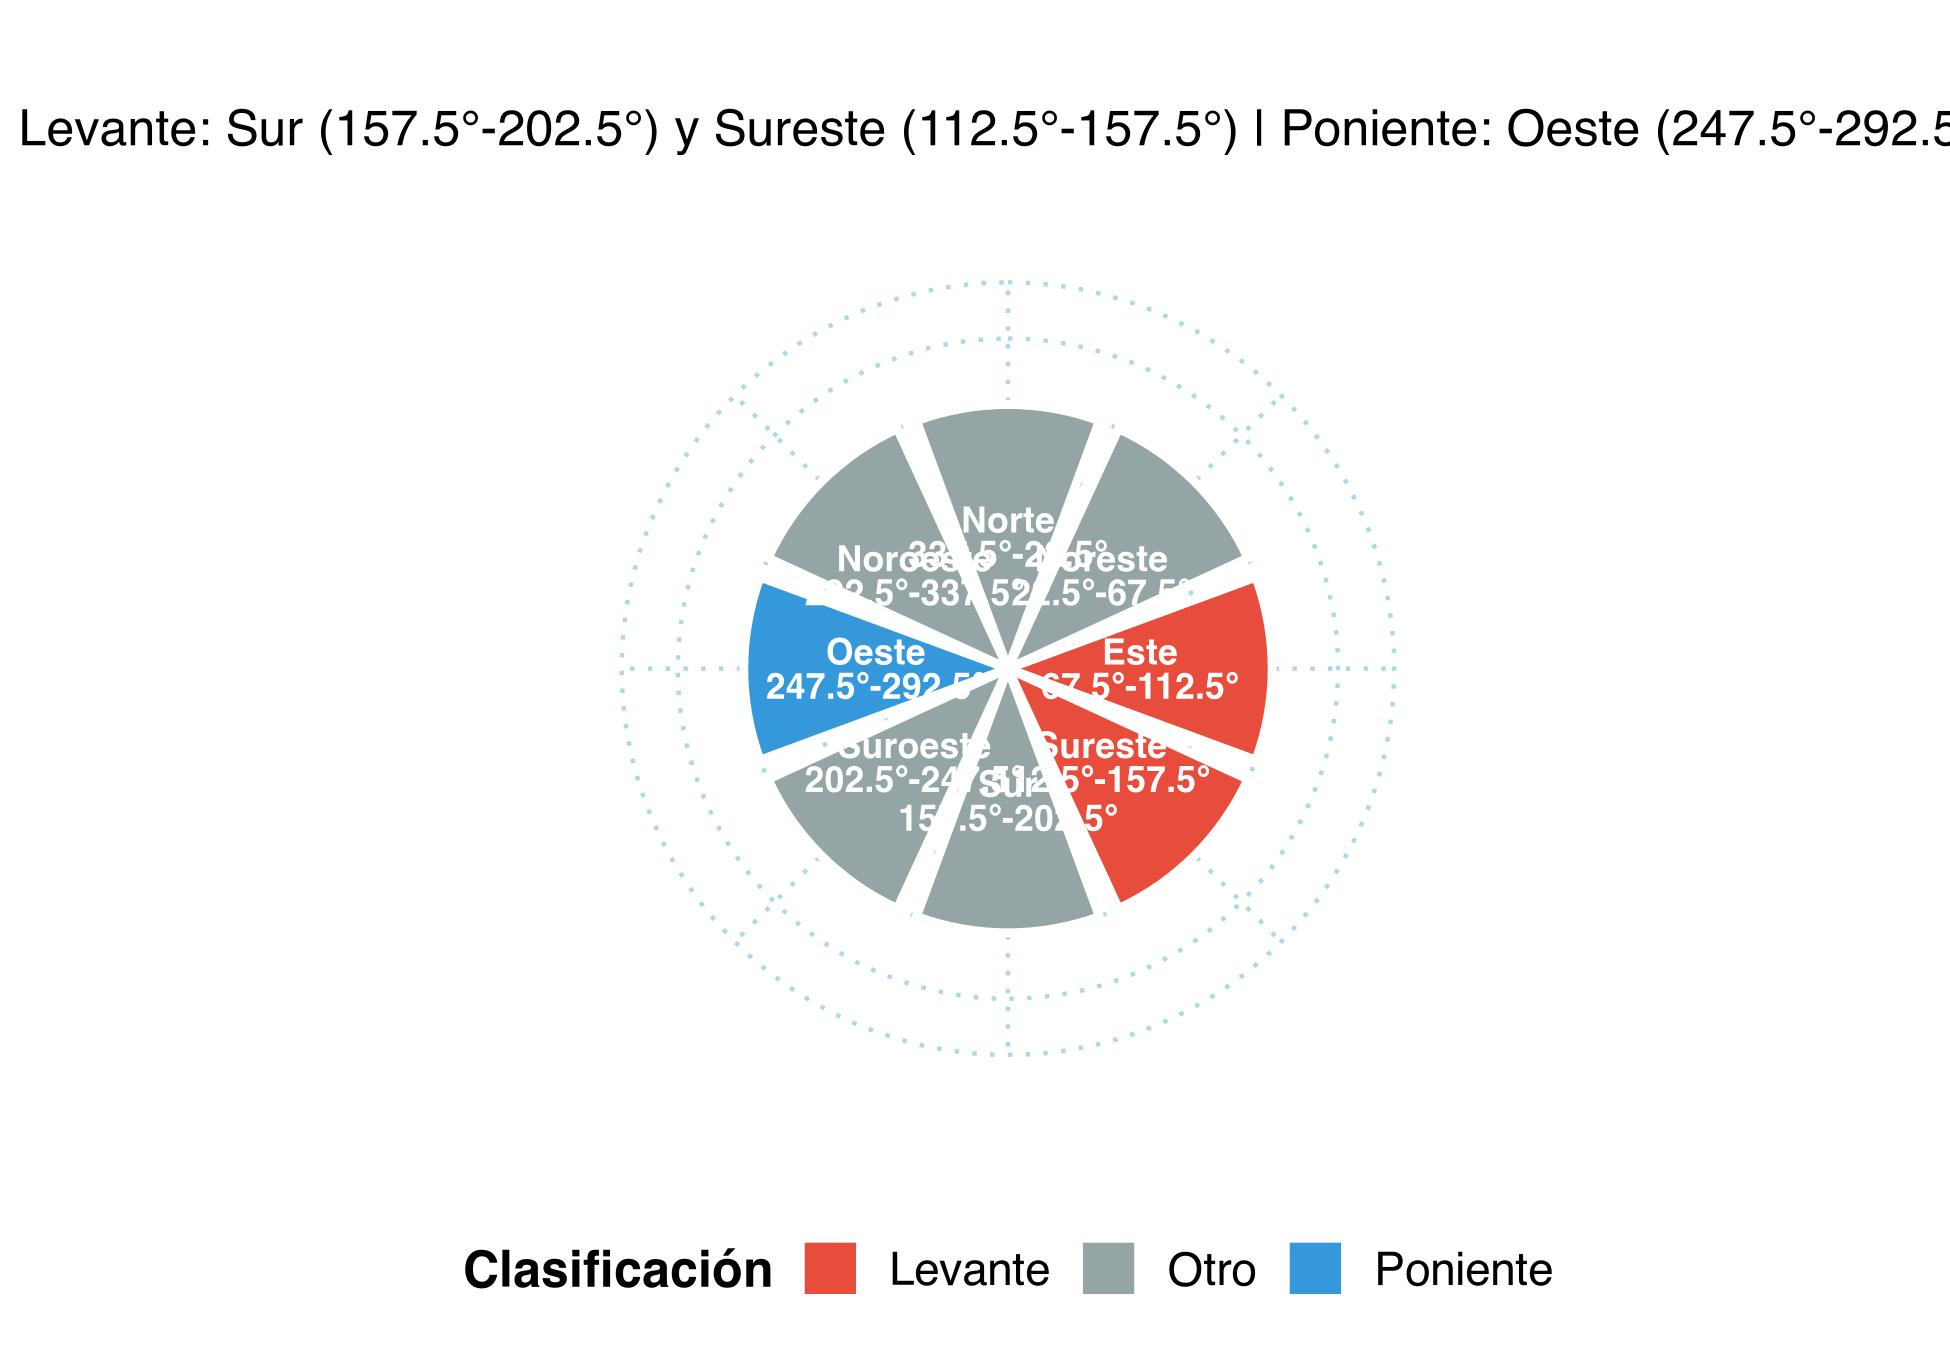
\includegraphics{Levante_Analisys_files/figure-latex/wind-rose-classification-1} 

}

\caption{Rosa de vientos mostrando la clasificación de sectores para Levante y Poniente}\label{fig:wind-rose-classification}
\end{figure}

\begin{Shaded}
\begin{Highlighting}[]
\CommentTok{\# Clasificar los datos de viento}
\NormalTok{datos\_clasificados }\OtherTok{\textless{}{-}}\NormalTok{ datos\_limpios }\SpecialCharTok{\%\textgreater{}\%}
    \FunctionTok{mutate}\NormalTok{(}\AttributeTok{tipo\_viento =} \FunctionTok{case\_when}\NormalTok{(velocidad\_viento }\SpecialCharTok{\textgreater{}=}
        \DecValTok{4} \SpecialCharTok{\&}\NormalTok{ velocidad\_viento }\SpecialCharTok{\textless{}=} \DecValTok{40} \SpecialCharTok{\&}\NormalTok{ direccion\_grados }\SpecialCharTok{\textgreater{}=}
        \FloatTok{67.5} \SpecialCharTok{\&}\NormalTok{ direccion\_grados }\SpecialCharTok{\textless{}=} \FloatTok{157.5} \SpecialCharTok{\textasciitilde{}}
        \StringTok{"Levante"}\NormalTok{, velocidad\_viento }\SpecialCharTok{\textgreater{}=} \DecValTok{8} \SpecialCharTok{\&}
\NormalTok{        velocidad\_viento }\SpecialCharTok{\textless{}=} \DecValTok{40} \SpecialCharTok{\&}\NormalTok{ direccion\_grados }\SpecialCharTok{\textgreater{}=}
        \FloatTok{247.5} \SpecialCharTok{\&}\NormalTok{ direccion\_grados }\SpecialCharTok{\textless{}=} \FloatTok{292.5} \SpecialCharTok{\textasciitilde{}}
        \StringTok{"Poniente"}\NormalTok{, }\ConstantTok{TRUE} \SpecialCharTok{\textasciitilde{}} \StringTok{"Otro"}\NormalTok{))}
\end{Highlighting}
\end{Shaded}

\subsection{Análisis de frecuencias}\label{anuxe1lisis-de-frecuencias}

\subsubsection{Distribución de velocidades y direcciones}\label{distribuciuxf3n-de-velocidades-y-direcciones}

\begin{Shaded}
\begin{Highlighting}[]
\CommentTok{\# Función para clasificar en puntos}
\CommentTok{\# cardinales}
\NormalTok{puntos\_cardinales }\OtherTok{\textless{}{-}} \ControlFlowTok{function}\NormalTok{(grados) \{}
    \FunctionTok{case\_when}\NormalTok{(grados }\SpecialCharTok{\textgreater{}=} \FloatTok{337.5} \SpecialCharTok{|}\NormalTok{ grados }\SpecialCharTok{\textless{}}
        \FloatTok{22.5} \SpecialCharTok{\textasciitilde{}} \StringTok{"N"}\NormalTok{, grados }\SpecialCharTok{\textgreater{}=} \FloatTok{22.5} \SpecialCharTok{\&}\NormalTok{ grados }\SpecialCharTok{\textless{}}
        \FloatTok{67.5} \SpecialCharTok{\textasciitilde{}} \StringTok{"NE"}\NormalTok{, grados }\SpecialCharTok{\textgreater{}=} \FloatTok{67.5} \SpecialCharTok{\&}\NormalTok{ grados }\SpecialCharTok{\textless{}}
        \FloatTok{112.5} \SpecialCharTok{\textasciitilde{}} \StringTok{"E"}\NormalTok{, grados }\SpecialCharTok{\textgreater{}=} \FloatTok{112.5} \SpecialCharTok{\&}\NormalTok{ grados }\SpecialCharTok{\textless{}}
        \FloatTok{157.5} \SpecialCharTok{\textasciitilde{}} \StringTok{"SE"}\NormalTok{, grados }\SpecialCharTok{\textgreater{}=} \FloatTok{157.5} \SpecialCharTok{\&}\NormalTok{ grados }\SpecialCharTok{\textless{}}
        \FloatTok{202.5} \SpecialCharTok{\textasciitilde{}} \StringTok{"S"}\NormalTok{, grados }\SpecialCharTok{\textgreater{}=} \FloatTok{202.5} \SpecialCharTok{\&}\NormalTok{ grados }\SpecialCharTok{\textless{}}
        \FloatTok{247.5} \SpecialCharTok{\textasciitilde{}} \StringTok{"SW"}\NormalTok{, grados }\SpecialCharTok{\textgreater{}=} \FloatTok{247.5} \SpecialCharTok{\&}\NormalTok{ grados }\SpecialCharTok{\textless{}}
        \FloatTok{292.5} \SpecialCharTok{\textasciitilde{}} \StringTok{"W"}\NormalTok{, grados }\SpecialCharTok{\textgreater{}=} \FloatTok{292.5} \SpecialCharTok{\&}\NormalTok{ grados }\SpecialCharTok{\textless{}}
        \FloatTok{337.5} \SpecialCharTok{\textasciitilde{}} \StringTok{"NW"}\NormalTok{)}
\NormalTok{\}}

\CommentTok{\# Análisis de velocidades}
\NormalTok{datos\_vel }\OtherTok{\textless{}{-}}\NormalTok{ datos\_clasificados }\SpecialCharTok{\%\textgreater{}\%}
    \FunctionTok{filter}\NormalTok{(}\SpecialCharTok{!}\FunctionTok{is.na}\NormalTok{(velocidad\_viento)) }\SpecialCharTok{\%\textgreater{}\%}
    \FunctionTok{mutate}\NormalTok{(}\AttributeTok{clase\_velocidad =} \FunctionTok{cut}\NormalTok{(velocidad\_viento,}
        \AttributeTok{breaks =} \FunctionTok{seq}\NormalTok{(}\DecValTok{0}\NormalTok{, }\DecValTok{24}\NormalTok{, }\AttributeTok{by =} \DecValTok{3}\NormalTok{), }\AttributeTok{include.lowest =} \ConstantTok{TRUE}\NormalTok{,}
        \AttributeTok{right =} \ConstantTok{FALSE}\NormalTok{)) }\SpecialCharTok{\%\textgreater{}\%}
    \FunctionTok{count}\NormalTok{(clase\_velocidad) }\SpecialCharTok{\%\textgreater{}\%}
    \FunctionTok{mutate}\NormalTok{(}\AttributeTok{porcentaje =} \DecValTok{100} \SpecialCharTok{*}\NormalTok{ n}\SpecialCharTok{/}\FunctionTok{sum}\NormalTok{(n))}

\CommentTok{\# Gráfico 1: Velocidad media}
\NormalTok{g1 }\OtherTok{\textless{}{-}} \FunctionTok{ggplot}\NormalTok{(datos\_vel, }\FunctionTok{aes}\NormalTok{(}\AttributeTok{x =}\NormalTok{ clase\_velocidad,}
    \AttributeTok{y =}\NormalTok{ porcentaje)) }\SpecialCharTok{+} \FunctionTok{geom\_bar}\NormalTok{(}\AttributeTok{stat =} \StringTok{"identity"}\NormalTok{,}
    \AttributeTok{fill =} \StringTok{"skyblue"}\NormalTok{, }\AttributeTok{color =} \StringTok{"black"}\NormalTok{) }\SpecialCharTok{+}
    \FunctionTok{labs}\NormalTok{(}\AttributeTok{x =} \StringTok{"Velocidad Media (m/s)"}\NormalTok{, }\AttributeTok{y =} \StringTok{"Frecuencia \%"}\NormalTok{) }\SpecialCharTok{+}
    \FunctionTok{theme\_minimal}\NormalTok{(}\AttributeTok{base\_size =} \DecValTok{13}\NormalTok{)}

\CommentTok{\# Análisis de direcciones con tipos de}
\CommentTok{\# viento}
\NormalTok{datos\_dir }\OtherTok{\textless{}{-}}\NormalTok{ datos\_clasificados }\SpecialCharTok{\%\textgreater{}\%}
    \FunctionTok{filter}\NormalTok{(}\SpecialCharTok{!}\FunctionTok{is.na}\NormalTok{(direccion\_grados)) }\SpecialCharTok{\%\textgreater{}\%}
    \FunctionTok{mutate}\NormalTok{(}\AttributeTok{direccion\_cardinal =} \FunctionTok{puntos\_cardinales}\NormalTok{(direccion\_grados),}
        \AttributeTok{tipo\_viento =} \FunctionTok{case\_when}\NormalTok{(direccion\_cardinal }\SpecialCharTok{\%in\%}
            \FunctionTok{c}\NormalTok{(}\StringTok{"E"}\NormalTok{, }\StringTok{"SE"}\NormalTok{) }\SpecialCharTok{\textasciitilde{}} \StringTok{"Levante"}\NormalTok{, direccion\_cardinal }\SpecialCharTok{\%in\%}
            \FunctionTok{c}\NormalTok{(}\StringTok{"W"}\NormalTok{) }\SpecialCharTok{\textasciitilde{}} \StringTok{"Poniente"}\NormalTok{, }\ConstantTok{TRUE} \SpecialCharTok{\textasciitilde{}} \StringTok{"Otro"}\NormalTok{)) }\SpecialCharTok{\%\textgreater{}\%}
    \FunctionTok{count}\NormalTok{(direccion\_cardinal, tipo\_viento) }\SpecialCharTok{\%\textgreater{}\%}
    \FunctionTok{mutate}\NormalTok{(}\AttributeTok{porcentaje =} \DecValTok{100} \SpecialCharTok{*}\NormalTok{ n}\SpecialCharTok{/}\FunctionTok{sum}\NormalTok{(n), }\AttributeTok{direccion\_cardinal =} \FunctionTok{factor}\NormalTok{(direccion\_cardinal,}
        \AttributeTok{levels =} \FunctionTok{c}\NormalTok{(}\StringTok{"N"}\NormalTok{, }\StringTok{"NE"}\NormalTok{, }\StringTok{"E"}\NormalTok{, }\StringTok{"SE"}\NormalTok{,}
            \StringTok{"S"}\NormalTok{, }\StringTok{"SW"}\NormalTok{, }\StringTok{"W"}\NormalTok{, }\StringTok{"NW"}\NormalTok{)))}

\CommentTok{\# Gráfico 2: Dirección cardinal con}
\CommentTok{\# colores por tipo de viento}
\NormalTok{g2 }\OtherTok{\textless{}{-}} \FunctionTok{ggplot}\NormalTok{(datos\_dir, }\FunctionTok{aes}\NormalTok{(}\AttributeTok{x =}\NormalTok{ direccion\_cardinal,}
    \AttributeTok{y =}\NormalTok{ porcentaje, }\AttributeTok{fill =}\NormalTok{ tipo\_viento)) }\SpecialCharTok{+}
    \FunctionTok{geom\_bar}\NormalTok{(}\AttributeTok{stat =} \StringTok{"identity"}\NormalTok{, }\AttributeTok{color =} \StringTok{"black"}\NormalTok{) }\SpecialCharTok{+}
    \FunctionTok{labs}\NormalTok{(}\AttributeTok{x =} \StringTok{"Dirección de Procedencia"}\NormalTok{,}
        \AttributeTok{y =} \StringTok{"Frecuencia \%"}\NormalTok{) }\SpecialCharTok{+} \FunctionTok{scale\_fill\_manual}\NormalTok{(}\AttributeTok{values =} \FunctionTok{c}\NormalTok{(}\AttributeTok{Levante =} \StringTok{"\#d62728"}\NormalTok{,}
    \AttributeTok{Poniente =} \StringTok{"\#1f77b4"}\NormalTok{, }\AttributeTok{Otro =} \StringTok{"\#95A5A6"}\NormalTok{)) }\SpecialCharTok{+}
    \FunctionTok{coord\_polar}\NormalTok{(}\AttributeTok{theta =} \StringTok{"x"}\NormalTok{) }\SpecialCharTok{+} \FunctionTok{theme\_minimal}\NormalTok{(}\AttributeTok{base\_size =} \DecValTok{13}\NormalTok{) }\SpecialCharTok{+}
    \FunctionTok{theme}\NormalTok{(}\AttributeTok{legend.position =} \StringTok{"bottom"}\NormalTok{)}

\NormalTok{gridExtra}\SpecialCharTok{::}\FunctionTok{grid.arrange}\NormalTok{(g1, g2, }\AttributeTok{ncol =} \DecValTok{2}\NormalTok{)}
\end{Highlighting}
\end{Shaded}

\begin{figure}[h]

{\centering 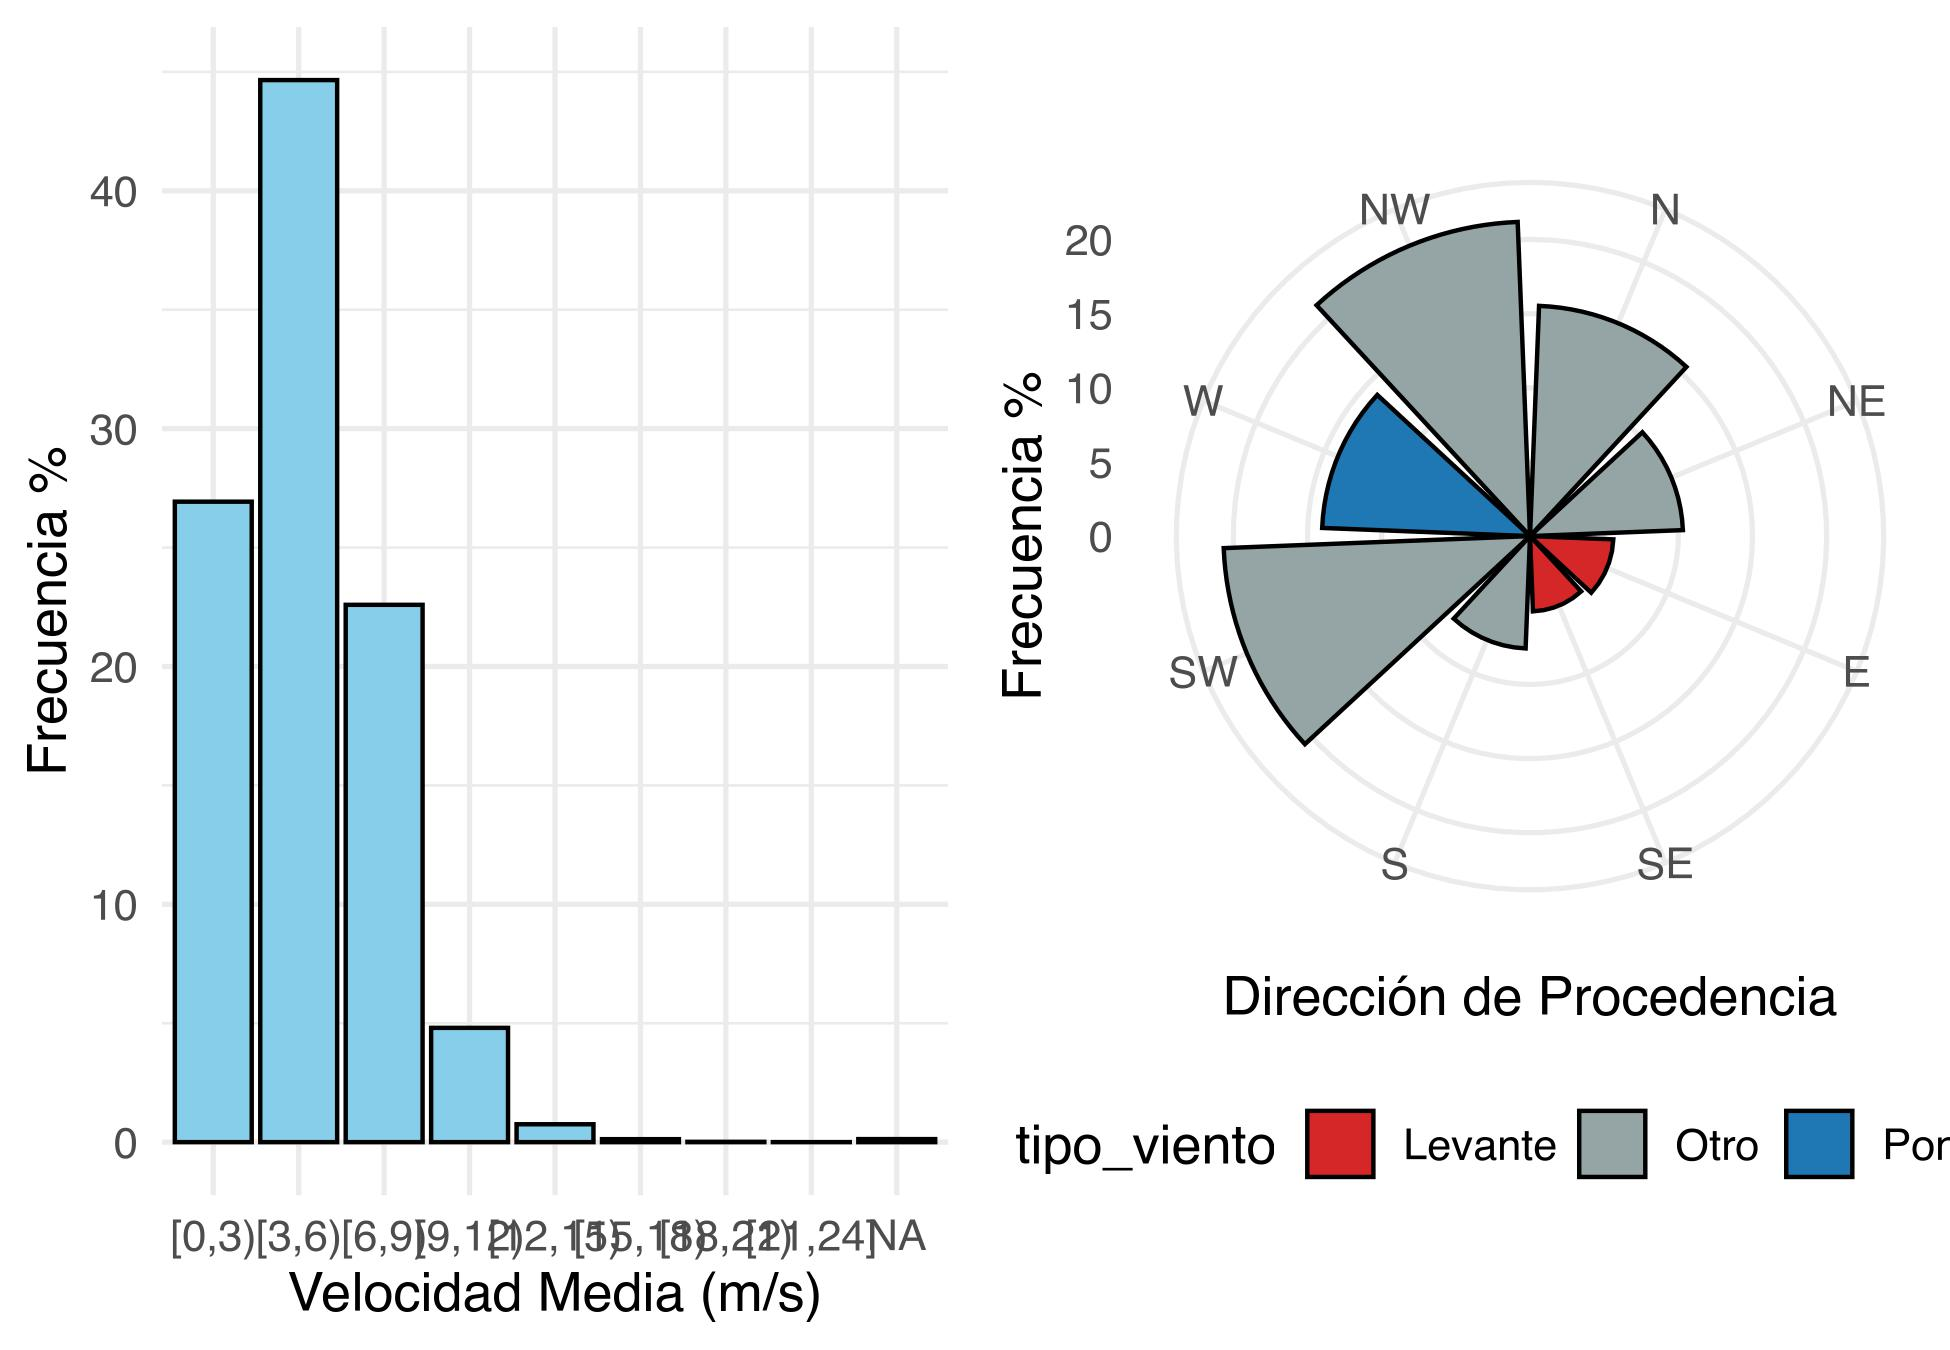
\includegraphics{Levante_Analisys_files/figure-latex/frequency-analysis-1} 

}

\caption{Distribución de velocidades del viento y frecuencia por dirección cardinal}\label{fig:frequency-analysis}
\end{figure}

\subsection{Análisis de eventos de viento}\label{anuxe1lisis-de-eventos-de-viento}

\subsubsection{Duración e intensidad de episodios}\label{duraciuxf3n-e-intensidad-de-episodios}

\end{document}
